\usetikzlibrary{shapes.geometric}
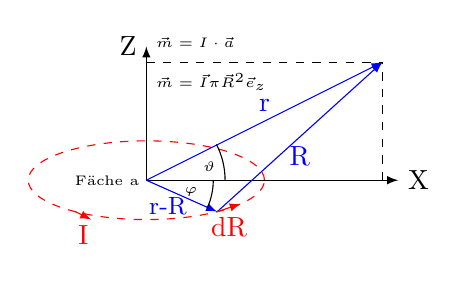
\begin{tikzpicture}
    %Elipse
    \node[ellipse,
        draw = red,
        dashed,
        minimum width = 3cm,
        minimum height = 1cm] (e) at (0,0) {};
    %Koordinaten Achsen
    \draw[-latex](0,0)--(3.2,0) node[right]{X};
    \draw[-latex](0,0)--(0,1.7) node[left]{Z};
    %Pfeile
    \draw[-latex, blue](0,0)--(3,1.5) node[above, midway]{r};
    \draw[-latex, blue](0.9,-0.4)--(3,1.5) node[below, midway]{R};
    \draw[-latex, blue](0,0) -- (0.9,-0.4) node[midway, below, yshift=3pt, xshift=-5pt]{\small{r-R}};
    \draw[-latex, red](0.9,-0.4)--(1.2,-0.3) node[midway, below]{dR};
    \draw[-latex, red](-0.9,-0.4)--(-0.7,-0.5) node[midway, below]{I};
    %Winkel
    \draw[-] (27:1) arc (27:0:1)
        node[left, yshift=5] {\tiny{$\vartheta$}};
    \draw[-] (0:0.85) arc (0:-25:0.85)
        node[left, yshift=6] {\tiny{$\varphi$}};
    %Legende
    \node[right] at (0,1.25){\tiny{$\vec{m}=\vec{I}\pi\vec{R}^2\vec{e}_z$}};
    \node[right] at (0,1.75){\tiny{$\vec{m}=I\cdot\vec{a}$}};
    \node[] at (-0.5,0){\tiny{Fäche a}};
    %Linien
    \draw[dashed](3,0)--(3,1.5);
    \draw[dashed](0,1.5)--(3,1.5);
\end{tikzpicture}
